\documentclass[border=10pt]{standalone}

\usepackage{tikz}
\usepackage{tikzsymbols}
\usetikzlibrary{calc,patterns,shapes.geometric}

\def\centerarc[#1](#2)(#3:#4:#5){\draw[#1] ($(#2)+({#5*cos(#3)},{#5*sin(#3)})$) arc (#3:#4:#5);}

\begin{document}
	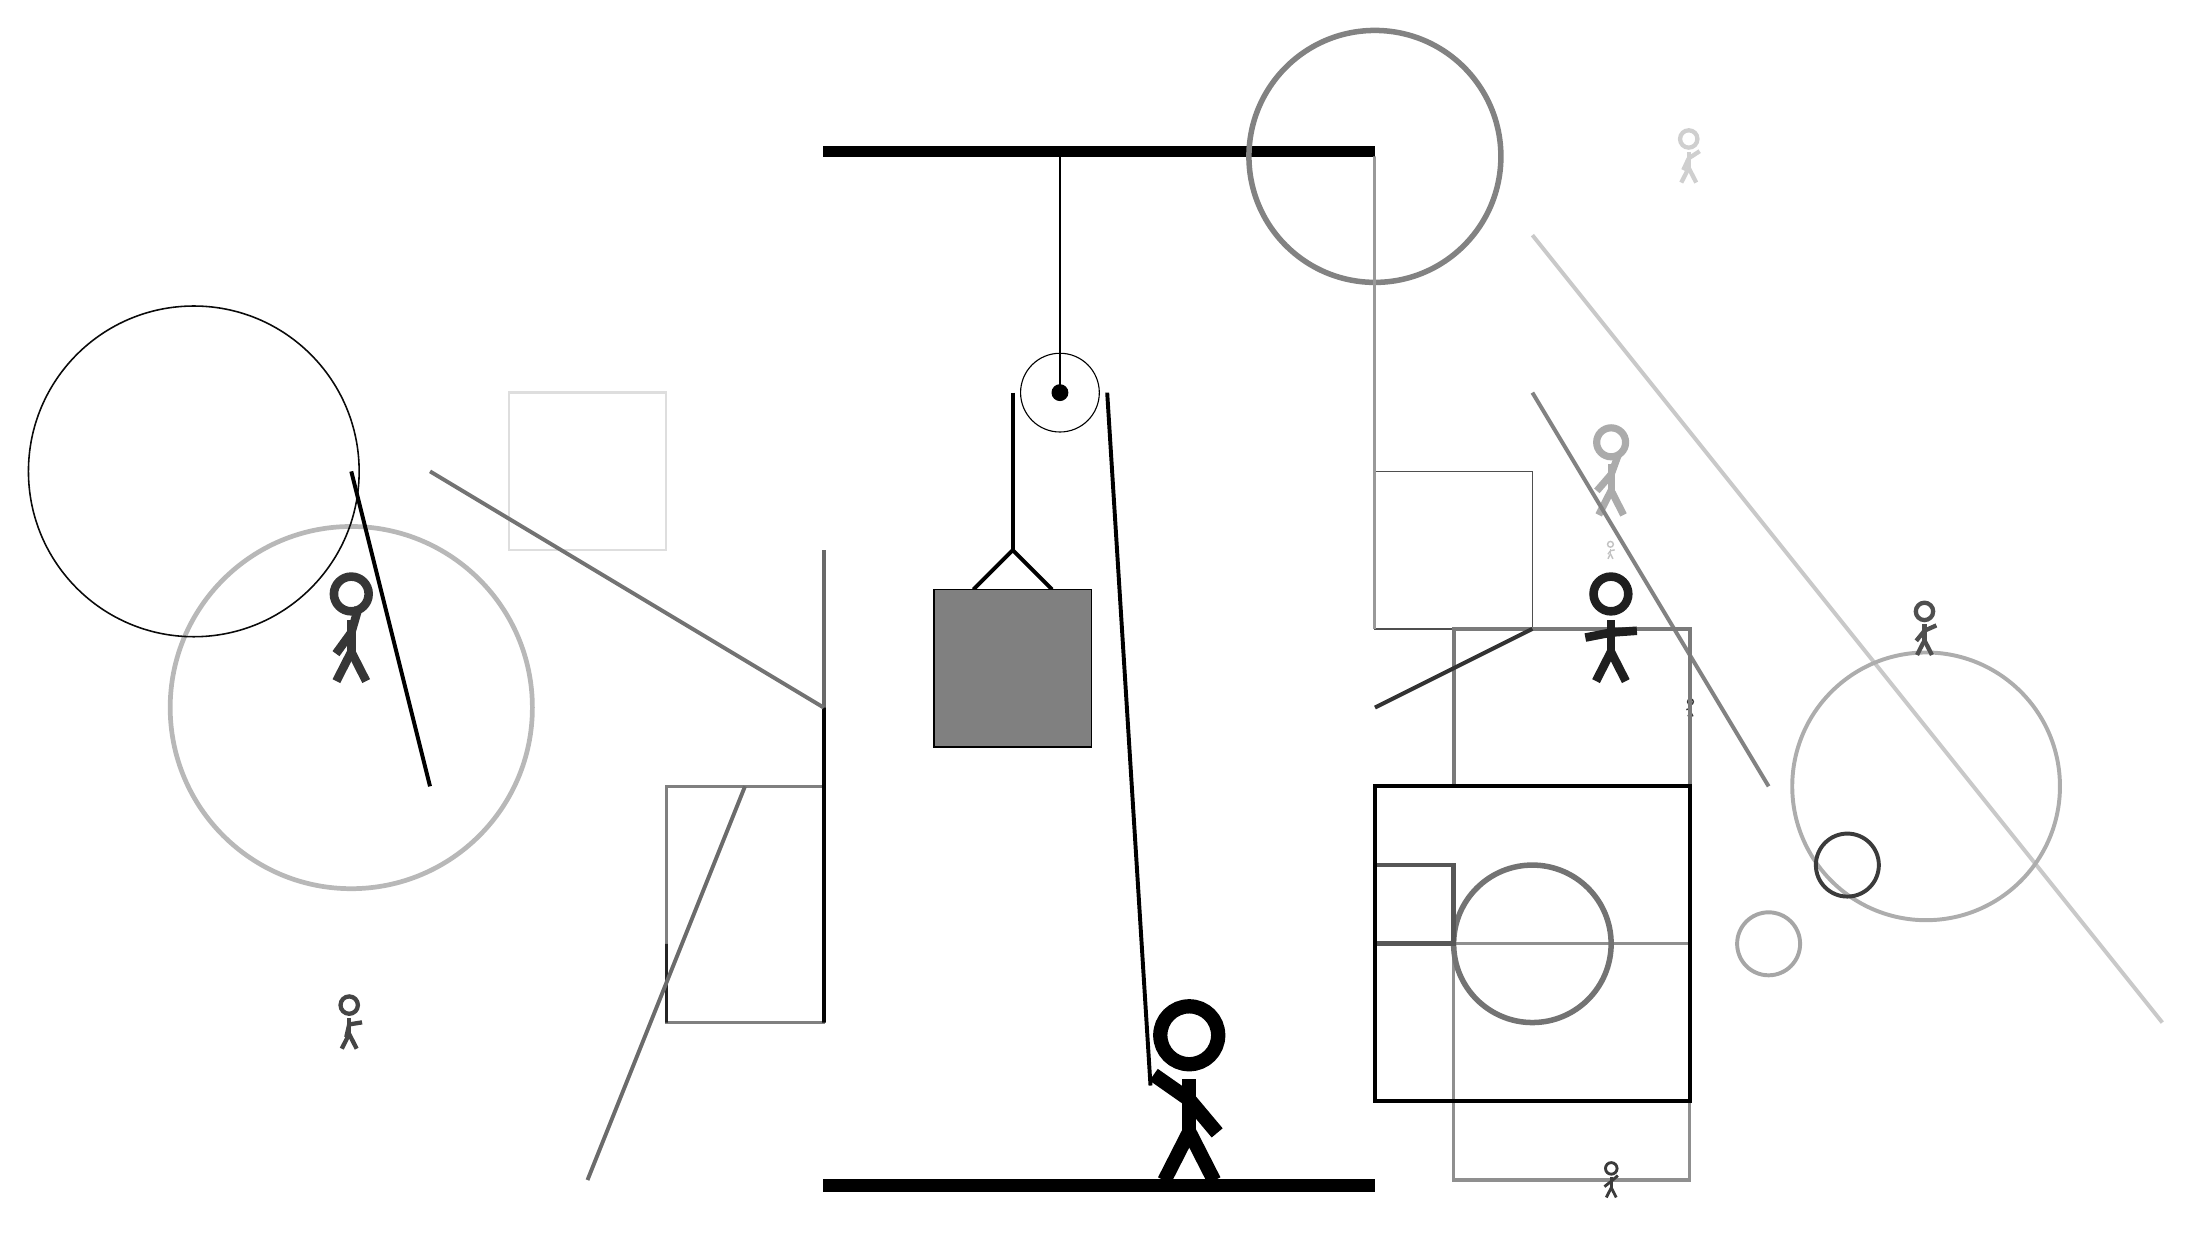
\begin{tikzpicture}
		%%%%% START %%%%%
		
		\draw[fill=black] (-2, 10) rectangle (5, 10.125);
		
		\draw (1, 7) circle (0.5);
		\draw[fill=black] (1, 7) circle (0.1);
		\draw (1, 10) -- (1, 7);
		
		\draw[line width=0.5mm] (-0.1, 4.5) -- (0.4, 5.0) -- (0.9, 4.5);
		\draw[fill=black!50] (-0.6, 4.5) rectangle (1.4, 2.5);
		
		\draw[line width=0.5mm] (0.4, 7) -- (0.4, 5.0);
		\centerarc[line width=0.5mm](1, 7)(0:180:0.6);
		\draw[line width=0.5mm](1.6, 7) -- (2.15, -1.8);
		
		\node at (2.6, -1.9) {\Strichmaxerl[10][-35][-50]};
		
		\draw [line width=0.5mm, color=black!35](10, 0) circle (0.4);
		
		\draw[line width=0.5mm, color=black!59](-2, 5) -- (-2, 1);
		\node[line width=0.6mm, color=black!33] at (8, 6) {\Strichmaxerl[5][49][70]};
		\node[line width=0.7mm, color=black!73] at (-8, -1) {\Strichmaxerl[3][77][9]};
		\draw[line width=0.4mm, color=black!50] (-4, 2) rectangle (-2, -1);
		
		\draw [line width=0.4mm, color=black!43](6, 7) circle (0.0);
		\draw[line width=0.5mm, color=black!21](7, 9) -- (15, -1);
		
		\node[line width=0.5mm, color=black!19] at (9, 10) {\Strichmaxerl[3][65][33]};
		\draw [line width=0.6mm, color=black!28](-8, 3) circle (2.3);
		
		\draw[line width=0.2mm, color=black!69] (5, 6) rectangle (7, 4);
		\node[line width=0.7mm, color=black!79] at (-8, 4) {\Strichmaxerl[6][54][74]};
		\node[line width=0.5mm, color=black!24] at (8, 5) {\Strichmaxerl[1][55][12]};
		\draw [line width=0.2mm, color=black!96](-10, 6) circle (2.1);
		
		\draw [line width=0.7mm, color=black!49](5, 10) circle (1.6);
		\draw [line width=0.5mm, color=black!32](12, 2) circle (1.7);
		\draw[line width=0.4mm, color=black!40] (5, 10) rectangle (5, 4);
		
		\draw[line width=0.4mm, color=black!86] (-4, 0) rectangle (-4, -1);
		\draw[line width=0.3mm, color=black!13] (-4, 7) rectangle (-6, 5);
		\draw[line width=0.5mm, color=black!98] (-2, -1) rectangle (-2, 3);
		\node[line width=0.5mm, color=black!78] at (9, 3) {\Strichmaxerl[1][20][81]};
		\draw[line width=0.4mm, color=black!44] (6, -3) rectangle (9, 0);
		\draw[line width=0.5mm, color=black!44] (5, -2) rectangle (5, 0);
		\draw[line width=0.5mm, color=black!55](-7, 6) -- (-2, 3);
		\draw[line width=0.5mm, color=black!49](7, 7) -- (10, 2);
		\draw [line width=0.7mm, color=black!55](7, 0) circle (1.0);
		
		\node[line width=0.5mm, color=black!77] at (8, -3) {\Strichmaxerl[2][38][41]};
		
		\draw[line width=0.5mm, color=black!52] (6, 4) rectangle (9, 2);
		\node[line width=0.7mm, color=black!88] at (8, 4) {\Strichmaxerl[6][11][4]};
		\draw[line width=0.6mm, color=black!66] (6, 1) rectangle (5, 0);
		
		\draw[line width=0.5mm, color=black!100](-7, 2) -- (-8, 6);
		\draw [line width=0.5mm, color=black!77](11, 1) circle (0.4);
		
		\node[line width=0.4mm, color=black!69] at (12, 4) {\Strichmaxerl[3][51][24]};
		\draw[line width=0.5mm, color=black!100] (5, -2) rectangle (9, 2);
		
		\draw[line width=0.5mm, color=black!80](5, 3) -- (7, 4);
		\draw[line width=0.5mm, color=black!58](-5, -3) -- (-3, 2);
		
		\draw[fill=black] (-2, -3) rectangle (5, -3.15);
		
		%%%%% END %%%%%
	\end{tikzpicture}
\end{document}